\chapter{Introduction}
\label{ch:Introduction}

\begin{comment}
\setlength{\epigraphwidth}{0.6\textwidth}
\setlength{\epigraphrule}{0.1pt}
%\epigraphhead[70]{%
    \epigraph{It would probably be oversimplifying the
matter,\\but I am strongly tempted to say,\\ ``All life is nucleic acid; the rest is
commentary''.}{\cite{asimov:WrongRel}}%
%}
\end{comment}


\begin{comment}
When Asimov concluded with these words his chapter ``Beginning with bone'',
scientists had already started unfolding one of the most mesmerising biological
mystery: how does the Nature manage and organise the production of specific
effectors in specific locations. In other words how from one cell
\TK{revoir cette phrase: idea initiale pourquoi
organisme A different
de B, ou un foie et un foie et pas un coeur + comment d'une cellule-oeuf on a un
organisme complet qui se creée... ne pas s'étendre dessus par contre}.\
Watson and Crick by publishing the double-helix structure of \DNA\
\mycite{DNA1953} unlocked our path to understand the natural ways of storing and
manipulating the information. As the whole past six decades were packed with major
discoveries and technological achievements, there are many, fascinating,
milestones that could be discussed.
The following pages present a summary of the facts and techniques
that form the biological and technical context of the work backing this thesis.

--- ici intro par rapport à Asimov et le fait que l'ADN est un 'blueprint' et qu'en
fonction du l'organe ou du develepment stage l'expression est régulé. On sait
maitenant que la régulation se passe à différent niveau.... finir peut être la
section sur Harvey qui a élucider la circulation sanguine car il a utilisé
l'observation et quantification du sang ---


As where the situation stands for now, we know that between the unique common
bluprint, which is the \DNA\ and the different phenotypes displayed by the tissues
comprising our bodies, they are many regulatory processes happening at different
layers (transcription, and translation).

 ### agent


\Rough{%
Gene expression, transcription, translation, regulation at each stage,
expected and reported correlation between transcripts and proteins
Measuring transcript expression by RNAseq, wet-lab part, analysis methods,
available large scale datasets on human tissues
Measuring protein expression by MS, data analysis – spectral counts, top 3, etc,
available large scale datasets on human tissues
The problem of comparing and integrating independent datasets, EBI’s GXA \\ \\
key concepts: DNA storage, RNA transfert of information and regulation,
protein effectors ==\textgreater phenotype.\\ \\
%
Do not forget the (tissues) specifications and the structural functions. =\textgreater Embryology.\\ \\
%
introduction real possible start: la soupe primaire -\textgreater creation de RNA, aa,
oeuf/poule
premiere cellule, \ldots (lire Darwin, il y a ptet moyen d ajouter une citation ou
quelque chose.%
}

\begin{itemize}
    \item Proteomics messy and noisy, challenging \ldots
    \item Transcriptomics seem a good proxy to study the phenotype => one kind of molecule made of the same pieces.
    \item Technology improved a lot from the microarrays to sequencing.
\end{itemize}

\end{comment}


\section{Diversity and universality of Life}



%\TK{Soupe primaire experience du Chimiste}
\TK{The central dogma of Molecular biology} => Crick describes the cycle

\fixme{Add references on replications, not going into that one}

\subsection{Translation + Regulation}

\subsection{Translation + Regulation}

Just so that the next part of the chapter got a OK presentation:
\begin{itemize}
    \item \gls{ncRNA}
    \item \gls{tRNA}
    \item \gls{miRNA}
    \item \gls{snRNA}
    \item \gls{scaRNA}
    \item \gls{snoRNA}
    \item \gls{scRNA}
\end{itemize}

\TK{Assumption mRNA and proteins : highly correlated [find references]}


\section{Capturing the expression in the laboratory}

Biological research uses mainly two approaches to
study the cell life intricacy and its underlying mechanisms.\\
The oldest approach is descriptive:


Small bits: corrections for Rnaseq are already part of the analysis and
requires often as much flair than skills.
Contrarily to \Dnaseq\ where corrections can be applied \TK{add reference} and
then the analysis be done, in Rnaseq each analysis requires a set of conform
quantification and normalisation methods.
While, there are quite established protocols for differential expression analysis,
there are presently many other downstream analyses that are cumbersome
and/or not settled yet. This is the case for this study.


Corrections for Rnaseq are already part of the analysis and
requires often as much flair than skills.

The transcriptome is the total repertoire of transcripts (\ie\ \glspl{RNA}
molecules) expressed in a cell or tissue at a given time and condition. Unlike
the genome which is roughly identical regardless which cell of a particular
individual is considered, the transcriptome varies\ldots

\subsection{Transcriptome exploration with RNA sequencing}

\TK{history of \Rnaseq.}
In the past decade, \gls{RNA-Seq} technology has risen as the method of choice
for  transcriptome.

Many methods and technologies through the years but more recently, boom of study:
next generation sequencing (1st generation, 2nd generation and 3rd)\ldots So
much that now the expression doesn't mean anything.

Completion of the Human genome project : key changer: probes with microarrays
possible (as there were then template). Next key changer: shotgun sequencing
instead of Sanger sequencing (slow). + advance in computer science: needs of
parallelisation and storage.

So, In 2008, shift from microarrays to \Rnaseq.

\clearpage

In the following section, I introduce the typical steps of the required workflow
to study the transcriptome through sequencing on an Illumina platform. In fact,
while not by conscious design, all the transcriptomes analysed in this thesis are
the product of Illumina sequencing. It is not surprising as Illumina was by far
the most popular platform for the last decade. Indeed, Illumina proposes a very
good ratio between the accuracy and the fact that it achieves the highest
throughput and the lowest per-base cost \mycite{IlluminaCheap}.

Experimental protocols for other platforms will need various and specific
modifications that are outside of the realm of this thesis and thus will not be
cover here. More details on the other main sequencing platforms and their
relevant protocols can be found in \cite{rnaseqProtocols} review paper or at the
online resource ``RNA-seqlopedia'' \mycite{rnaseqlopedia}.

As I discuss the concepts behind the Illumina sequencing technology and the
most common related methods to process it, I will emphasise the approaches and
the tools I used to estimate the gene expression levels from raw nucleotide
sequences.

\Cref{fig:OverviewRnaseqPrepSeq} presents an overview of the typical steps of a
\Rnaseq\ workflow from the libraries preparation to the sequencing.

\begin{figure}
    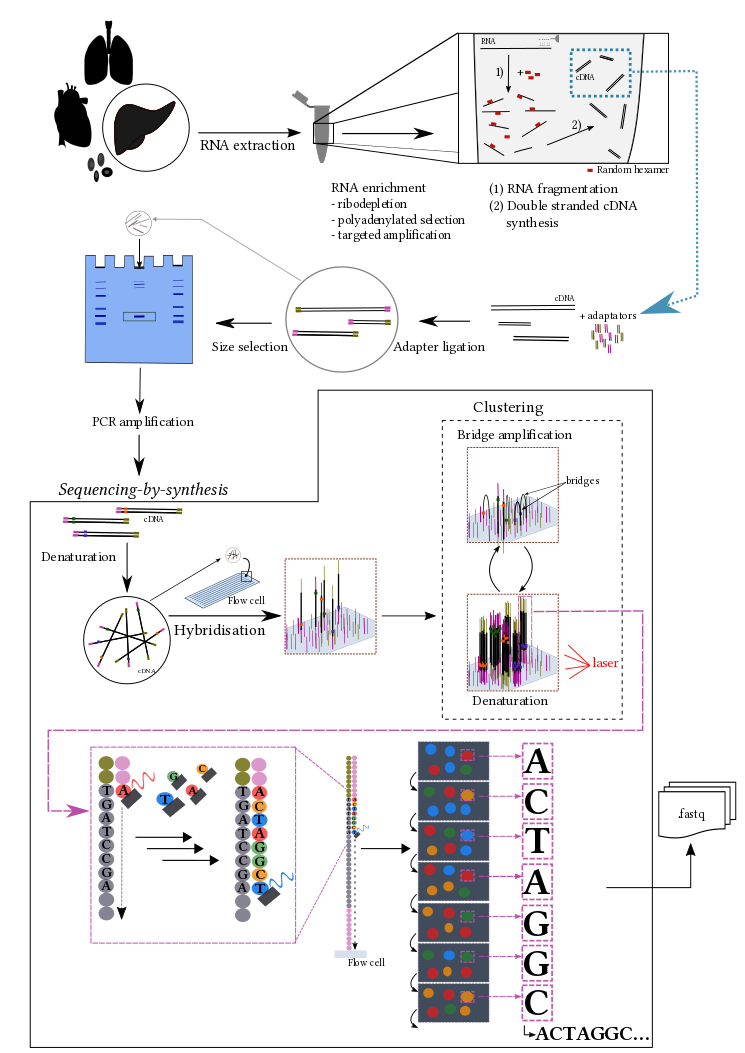
\includegraphics[scale=0.60]{introduction/IntroWorkflow}\centering
    \caption[Overview of a \Rnaseq\ workflow: library preparation
    and sequencing]{\label{fig:OverviewRnaseqPrepSeq}\textbf{Overview of
    a typical \Rnaseq\ workflow:
    library preparation and sequencing}}
\end{figure}

\NB Albeit the collection and the conservation of the samples prior to the
\gls{RNA} extraction most definitely affects the final estimations,
I will let aside these steps from my review.

\subsubsection{Library preparation}

The first step of a typical \Rnaseq\ workflow is the preparation of \gls{cDNA}
libraries from the starting material. This step and the sequencing itself are
the most platform dependent parts of the overall protocol. Indeed, contingently
on to the sequencing principle they rely, the sequencers need the libraries to
be fixed and loaded differently.

\minisec{\gls{RNA} extraction}
There are many methods to extract \glspl{RNA} from the primary samples and they
are commonly standardised. Indeed, regarding the type of biological samples,
the \glspl{RNA} of interest, the aim of the  study and the sequencing platform
used, there is one (or more) available commercial kit. These are designed in
a way to not interfere
with any of the later steps of the library preparation or with the sequencing
itself.
Without surprise, the choice of one kit (and hereby method of extraction)
over another can impact the final \Rnaseq\ data \mycite{RNAextraction}. The main
difference between the most widespread methods being the quantity of non-mature
\glspl{RNA} (\ie\ with longer intronic regions) detected whereby kit
has been used. However, the relative gene expression levels are similar.


\minisec{\gls{RNA} enrichment}

After extracting the \gls{RNA} from the cells or tissues,
the next step is to enrich the content of the samples with the \glspl{RNA}
of interest (\ie\ the concentration of the \glspl{RNA} of interest is increased
either by specifically selecting it or by removing other \glspl{RNA}). Indeed,
the \glspl{rRNA} are the most abundant type of \gls{RNA} in any cell. Even
though they are a very small part of the genome\footnote{For example,
\species{Homo sapiens}, there are only 568 genes (<1\%) that are described as
\gls{rRNA} out of the 63,898 annotated genes of the ENSEMBL database
(\hg{38.p10} - \ens{89}).}, they represent by their number 70\% or more of
the total population of \gls{RNA} \mycite{biochbook}.
Although there are interests to study \glspl{rRNA}, \mRNAs\ studies are more
popular and they only constitute about 3 to 5\% of the whole \gls{RNA} population
\mycite{molBiolCell}. Other studies research even scarcer kinds of \gls{RNA}.

There are typically three strategies to achieve \gls{RNA} enrichment:
either by polyA-selection, by ribodepletion or (more complex)
by targeted amplification. While these
approaches are insufficiently specific to select one particular kind of \gls{RNA}
or remove all \glspl{rRNA}, it eases and improves the downstream analyses.

\subminisec{PolyA-selection}
This strategy essentially targets the \mRNAs. It exploits the polyadenylated
tail at the 3' end of the \mRNAs\footnote{And a few other kinds of \gls{RNA},
\eg\ \glspl{lncRNA} \mycite{polyAlncRNA}} that is added
post-transcriptionally. In fact, magnetic beads supporting short
strings of thymine (oligo-dT) capture efficiently these \mRNAs\ while the others
are washed away \mycite{Mortazavi2008}.

This protocol is probably the most widespread one as it is the easiest and
cheapest to set up. A dataset produced following this protocol is known as
a \emph{polyA-selected} dataset.

\subminisec{Ribodepletion}
This strategy is preferred for the study of any \gls{ncRNA} or when researching
the interaction of \mRNAs\ with other \glspl{RNA} \mycite{ribodepletion}. This
strategy is in a way the reverse of the previous one as its also
uses magnetic beads, but this time to efficiently\footnote{ThermoFisher claims
that its RiboMinus protocol can remove till 99.99\% of the \glspl{rRNA}.}
target the unwanted \glspl{rRNA} as to remove from the sample.

The ribodepletion can also be achieved through ribonucleases. These enzymes
specifically digest \glspl{rRNA} and then \glspl{RNA} of interest can be retrieve
through size selection.

Datasets produced following a ribodepletion protocol are usually called
\emph{whole \gls{RNA}} or \emph{total \gls{RNA}} as a contrast to the
\emph{polyA-selected} ones.

\cite{castleData} created a total \gls{RNA} dataset but they use another
approach where they amplify \emph{every} other \gls{RNA} with the help of
specifically designed probes (see \Cref{subsec:castlepresentation}). Hence,
the protocol they have used is closer to the following one.

\subminisec{Targeted amplification}
Targeted amplifications rely on primers that would be designed to target (or
avoid as for \cite{castleData}) specific sequence motifs of the genome. Most
studies based on this type of approach are not referred as \Rnaseq\ studies, but
a name that is based on the kind of studied \gls{RNA} (\eg\ \gls{miRNA-Seq}) or
that emphasises the variation of the method (\eg\ Capture-Seq
\mycite{captureSeq}). Often, additional steps are required to prepare the
library comparatively to a polyA-selected or ribodepleted dataset.


\minisec{RNA fragmentation}
Most of the sequencing platforms\footnote{As for the Illumina platforms that have
produced the transcriptomic datasets studied in this thesis} require relatively
short (\eg\ 200 to 500 nt) length to sequence. Concomitantly, it also ensures
that the sampling along the \gls{RNA} is more uniform.
This fragmentation can be carry out via divalent cations hydrolysis or
nebullisation.

This step is sometimes performed after the \gls{cDNA} synthesis (see next section).
In those case, the \gls{cDNA} are fragmented by digestion with DNase I or by
sonication.

\minisec{Double-stranded cDNA synthesis}
There are sequencing technologies that can directly sequence \glspl{RNA}. Yet
most of the technologies handle only \gls{DNA}. Thus, the \gls{RNA}
molecules are used as a template for a retro-transcription involving
oligo-dTs or \emph{random} hexamer primers, respectively only for polyA-selected
datasets or any dataset (polyA-selected included). The set of \emph{random}
hexamer has been designed to cover the whole transcriptome. Unfortunately,
these \emph{random} hexamer primers have been proven to actually lack full
randomness \mycite{notSoRandom}.

At the end of the most common protocol, the order of synthesis of each \gls{cDNA}
strands is lost, \ie\ it is impossible to distinguish which of the \gls{cDNA}
strands has the same sequence than the original \gls{RNA}. Several techniques,
called \emph{strand-specific}, have been developed to compensate for this
(\mycite{strandSpecific}, \mycite{strandSpe}).

\minisec{Adapter ligation, PCR amplification and size selection}
After generating blunt edges by restriction digest of the \glspl{cDNA}, adapters
are ligated to their both ends. These adapters are ensuring the hybridisation of
the \glspl{cDNA} with the flow cell\footnote{The flow cell is the support of the
sequencing. It enables the parallelisation of the sequencing of millions of
\gls{DNA} fragments together as they are kept spatially separated. This was
allowed with the advent and optimisation of supported Chemistry.}
and are used for the following step as primers for the cluster amplification
happening \latin{in situ} on the flow cell.

Then, all the molecules are amplified by \gls{PCR}.

Finally, as the previous fragmentation step has created a greater range of length
that required by the typical sequencer machine (about 250 to 500 bp), a
size-selection is performed (per gel electrophoresis).

\TK{La suite au prochain numéro :p }

\subsubsection{Sequencing}

\minisec{Hybridisation}

\minisec{Cluster amplification}


\minisec{Sequencing-by-synthesis}


\minisec{Alternative preparation strategies}



\subsubsection{Read mapping strategies}

\minisec{Quality check, trimming and filtering}

\NB Generally, after the sequencer calls the reads, a first trimming removes
all the adaptors and barcodes needed by the sequencing protocols. Thus,
in principle, they are not to be found in raw data from repositories.
However, to avert any latter contingency, a research against
a list of the most common adaptors and an over-representation assessment of small
sequences (\emph{k-mers}) at each end of the reads is good practice.

\minisec{\latin{De novo} assembly}

\minisec{Read alignment}

\subminisec{Genome reference}

\subminisec{Transcriptome reference}



The quality assessment allows to remove any read (or part of it) that would
increase the complexity of the mapping step or skew the downstream analyses.

Whenever the overall quality of the samples allows it, it is best to discard very


Then, reads that present an overall quality score below a given threshold (10) are
fully discarded. Reads that have uncalled bases (\textsc{N}) are also discarded.
Since the quality decreases as the calling process progresses, all the reads are
trimmed to a same length\footnote{This is a requirement of some tools (mappers
in particular).} in a way to optimise the purity-length balance. The trimming has
to be less than 15\% of the original length. If needed, more reads are discarded
so the length is maximised.








\subsection{Transcriptomics Studies}
    \subsubsection{Main technologies}
While microarrays are measuring many \mRNAs\ at once, their number is limited,
     (ubsubsection{A typical sequencing workflow}
\subsection{Proteomics}
    \subsubsection{Main technologies}
    \subsubsection{Mass sprectrometry}

\section{Big studies, big data and Reproducibility}



\begin{comment}
\subsection{Reproducibility issues}
        \begin{itemize}
            \item{Different samples}
            \item{Technology: wet lab but also software: Rupgrade, ....}
            \item{missing meta-data}
        \end{itemize}
    \subsection{Main concerns}
        \subsubsection{Detection}
        \subsubsection{Quantification}
    \subsection{Consistency through biological layers}
\end{comment}


\subsection{Co-studies on Transcriptomics and Proteomics in the literature}
\subsection{EBI Expression Atlas or how integrating independent datasets }


\section{Aims of the thesis}

One main focus of my work for this thesis was to appraise the
consistency of findings that have been enlightened in normal Human tissues by
individual large scale transcriptomics and, more recently, large-scale
proteomics studies.

While the amount of data to process and integrate can be challenging,
paradoxically the data available to draw statistically significant conclusions
is often still too sparse. However, we do have enough to provide at least a
qualitative assessment of the consistency and evaluate the feasibility of a
quantitative assessment in general, if not, realise a quantitative integration
for a few key tissues.

\section{Achievements}
\begin{itemize}
    \item First time so many datasets have been reprocessed together with the
        same annotation and hence comparison are better (y'a le truc de chez Burges,
        mais ils se sont concentré sur une petite partie des genes)
    \item surtout comparison of Gtex and Uhlen (aussi approfondi)
    \item reprocessing of all the proteome untargeted in human
    \item comparison entre protein expression and 2 datasets (meilleur que le
        science report dans le sens où il y a pas de polémique
    \item siteweb//application de visualisaiton de la comparison
    \item liste croisé de tissues specifique et house keeping à travers datasets
        transcriptomic et protoemic
    \item attempt de normalisation basée sur les housekeepings
\end{itemize}


\section{Reproducibility vs. Repeatability}

\section{Comment preparer RNA-seq libraries?}

\section{Paired-end, Single-end}

\section{Experimental design}
\subsection{Technical replicates}
\subsection{Biological replicates}
pourquoi c'est important.
